\section{The parameter scan window}
\label{sec:scanwindow}
Related YouTube videos:
\begin{figure}[H]
\begin{tabular}{ c l }

\includegraphics[width=0.05\textwidth]{./images/youtube.png}
&
\href{https://www.youtube.com/watch?v=cpkPht-CKeE}{Using the parameter scan tool in OghmaNano}
\end{tabular}
\end{figure}

\vspace{0pt}
\noindent
\begin{minipage}{0.5\textwidth}
The most straight forward way to systematically vary a simulation parameter is to use the scan window. In this example we are going to systematic change the mobility of the active layer of a PM6:Y6 solar cell, you can find this example in the example simulations under \emph{Scripting and fitting/Scan demo (PMY:Y6 OPV)}. Once you have located this simulation and opened it, you then need to bring up the parameter scan window, this can be done by clicking on the \emph{Parameter scan} icon in the Automation ribbon (see Figure \ref{fig:parameter_scan_icon}).  Then make a new scan by clicking on the \emph{new scan} button (1) (In the example simulation this has already been done for you). Open the new scan by double clicking on the icon representing the scan (2), see figure \ref{fig:newscan}. This will bring up the scan window, see figure \ref{fig:newscanline}.
\end{minipage}% Don't leave empty lines and empty chars between minipages
\hspace{4pt}
\begin{minipage}[]{0.5\linewidth}
\centering
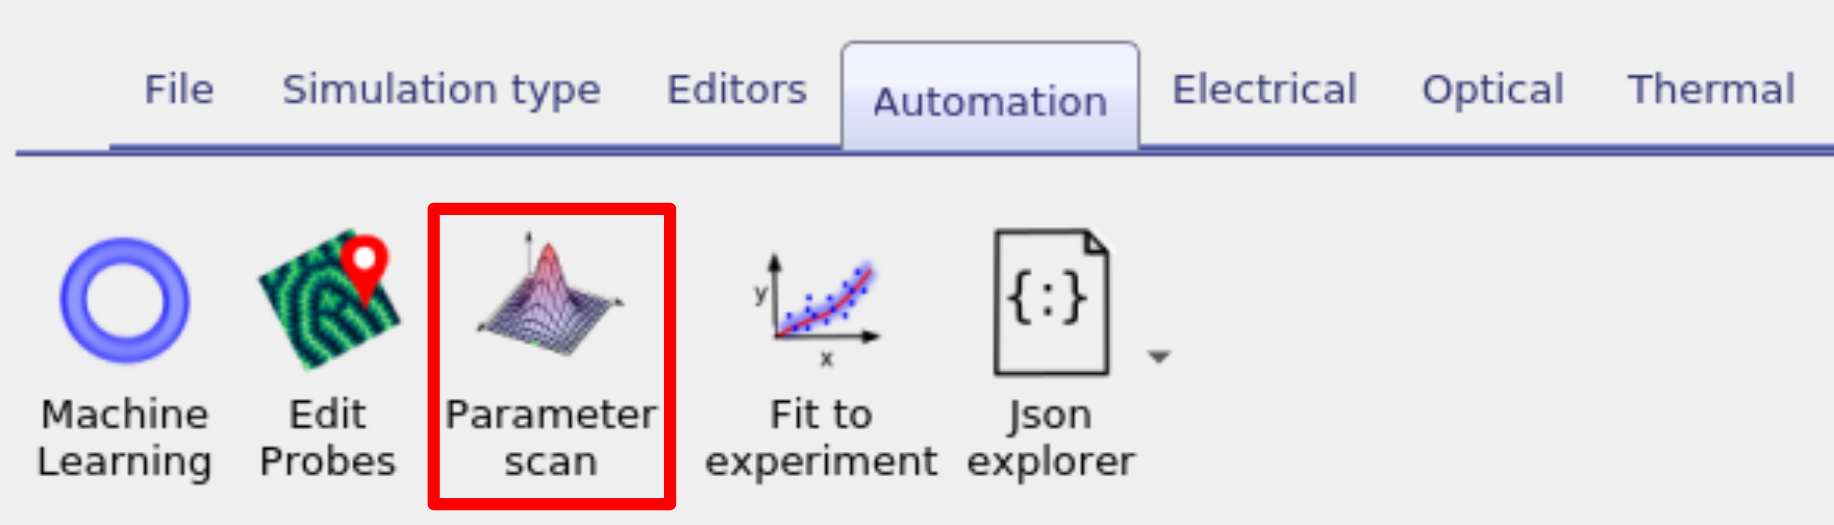
\includegraphics[width=\textwidth]{./images/param_scan.png}
\captionof{figure}{Step 1: Select the Parameter scan tool, to bring up the parameter scan window.}
\label{fig:parameter_scan_icon}

\centering
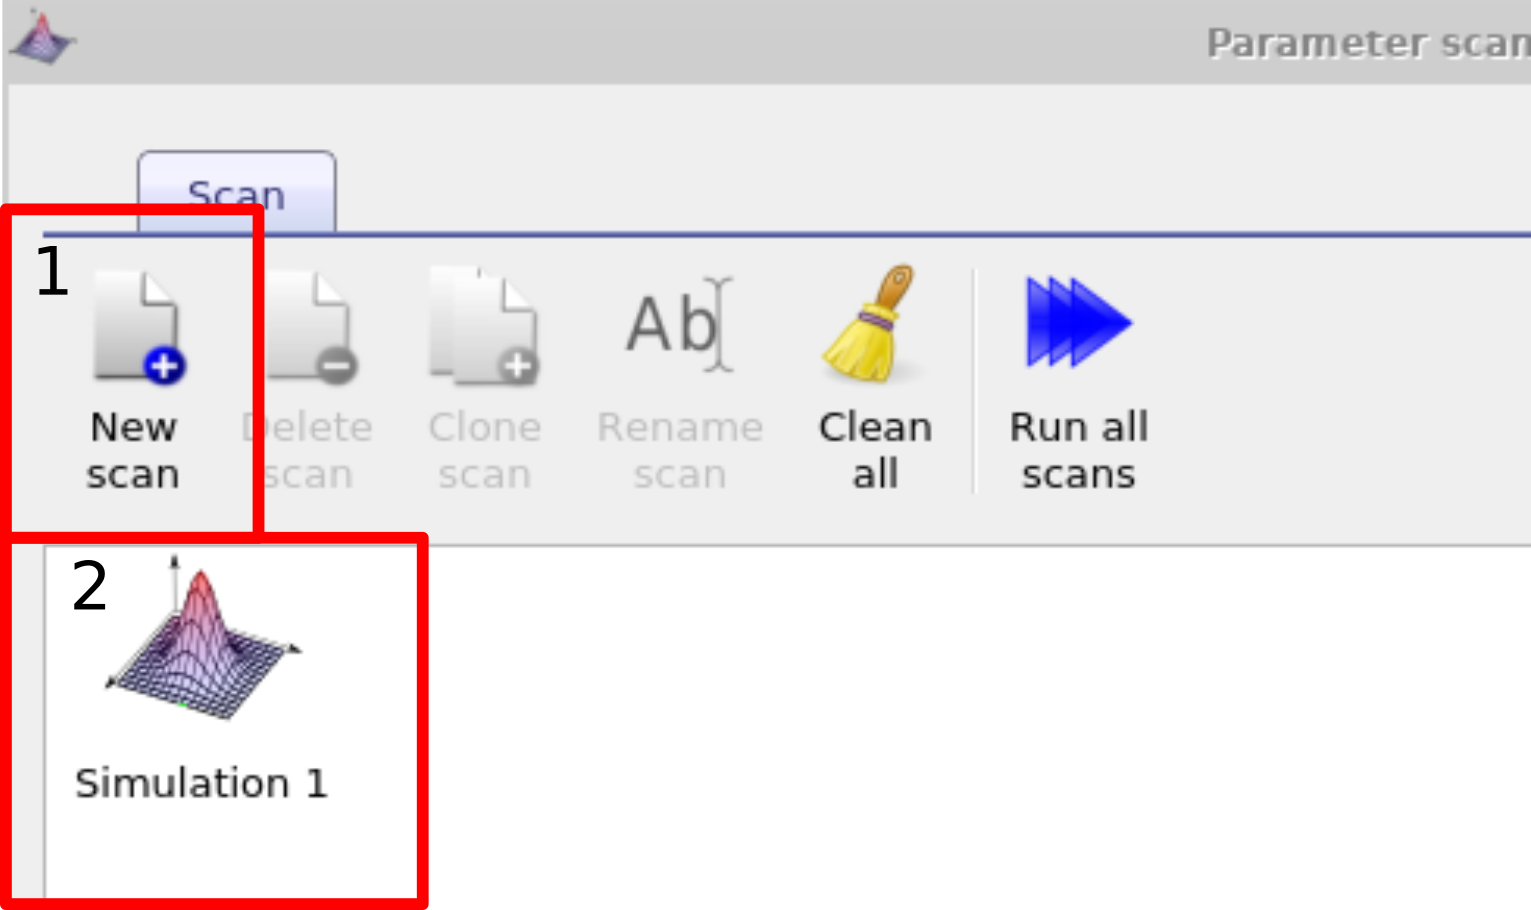
\includegraphics[width=\textwidth]{./images/param_scan_new.png}
\captionof{figure}{Step 2: Make a new parameter scan, then double click on it to open it.}
\label{fig:newscan}

\end{minipage}

\subsection{Changing one material parameter}
Once the \emph{scan window} has opened, make a new scan line by clicking on the the plus icon (1) in figure \ref{fig:newscanline}, then select this line so that it is highlighted (2), then click on the three dots (3) to select which parameter you want to scan. Again if you are using the example simulation this will already have been done for you.

\begin{figure}[H]
\centering
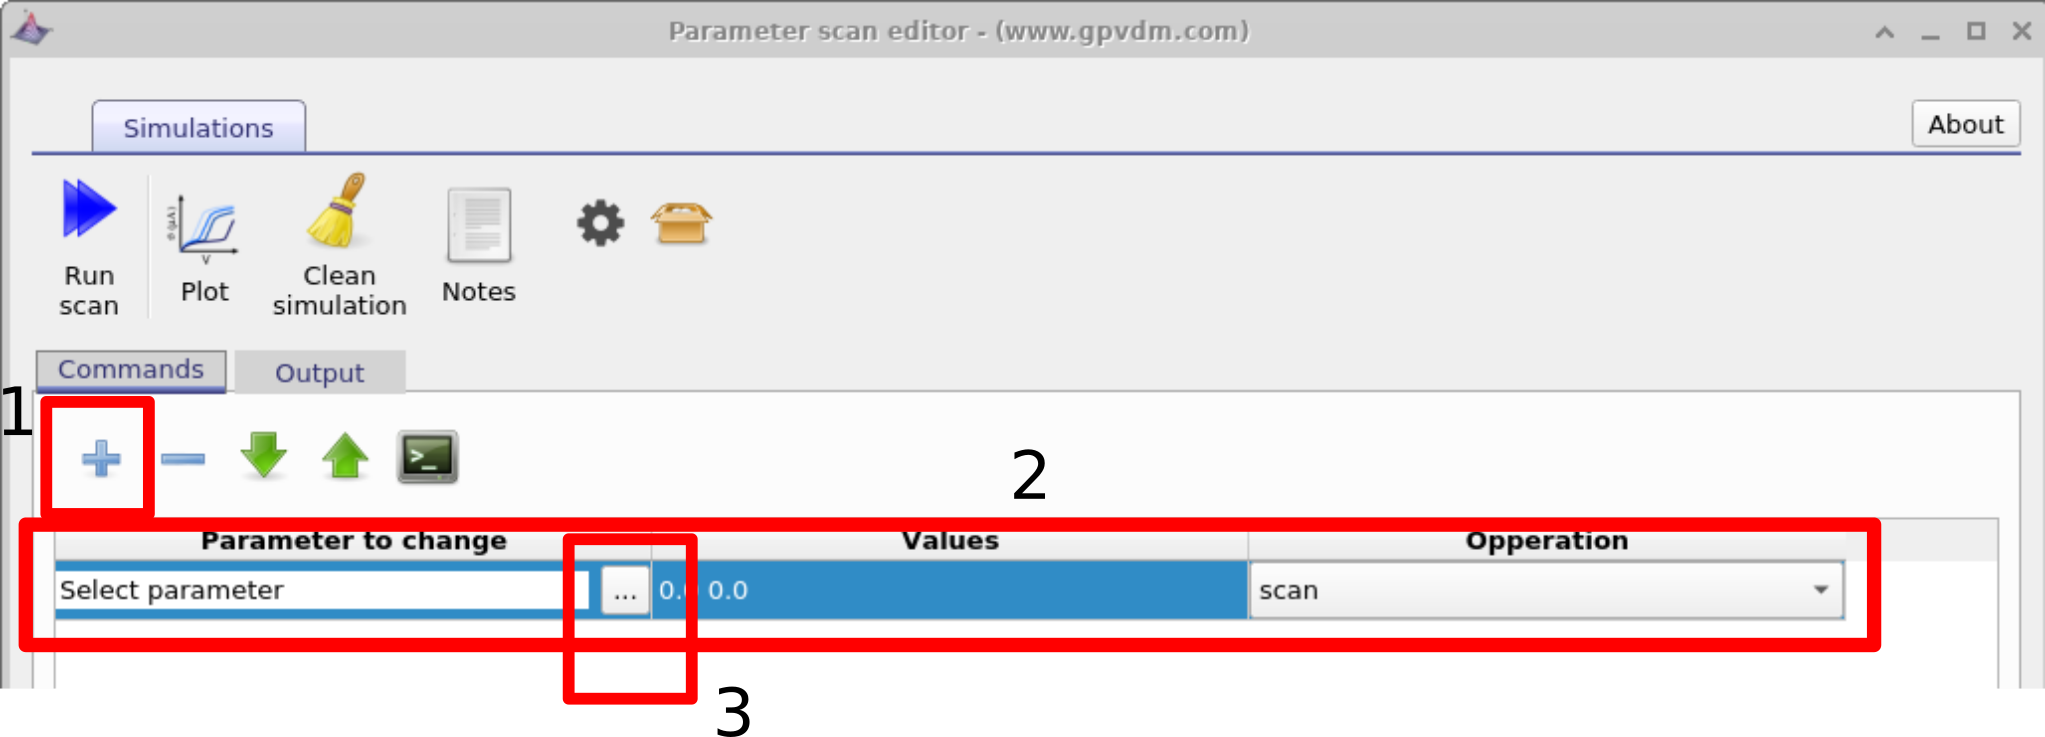
\includegraphics[width=\textwidth]{./images/param_scan_new_line.png}
\caption{Step 3: Add a 'scan line' to the scan.}
\label{fig:newscanline}
\end{figure}
\pagebreak
\noindent
\begin{minipage}{0.5\textwidth}

In this example we will be selecting the electron mobility of a PM6:Y6 solar cell. Do this by navigating to epitaxy$\rightarrow$ PM6:Y6$\rightarrow$ Drift diffusion$\rightarrow$ Electron mobility y. Highlight the parameter and then click OK. This should then appear in the scan line. The meaning of \emph{epitaxy$\rightarrow$ PM6:Y6$\rightarrow$ Drift diffusion$\rightarrow$Electron mobility y} will now be explained below:

\begin{itemize}
  \item epitaxy: All parameters in the .oghma file are exposed via the parameter selection window see \ref{fig:scanselect}. This file is a tree structure, see \ref{sec:fileformat}. The device structure is defined under the heading epitaxy.
  \item PM6:Y6: Under epitaxy each layer of the device is given by its name. The active layer in this device is called PM6:Y6, if your active layer was called Perovskite or P3HT:PCBM you would have selected this instead.
  \item Drift diffusion: All electrical parameters are stored under the sub heading \emph{drift diffusion}.
\end{itemize}

\end{minipage}% Don't leave empty lines and empty chars between minipages
\hspace{4pt}
\begin{minipage}[]{0.5\linewidth}
\centering
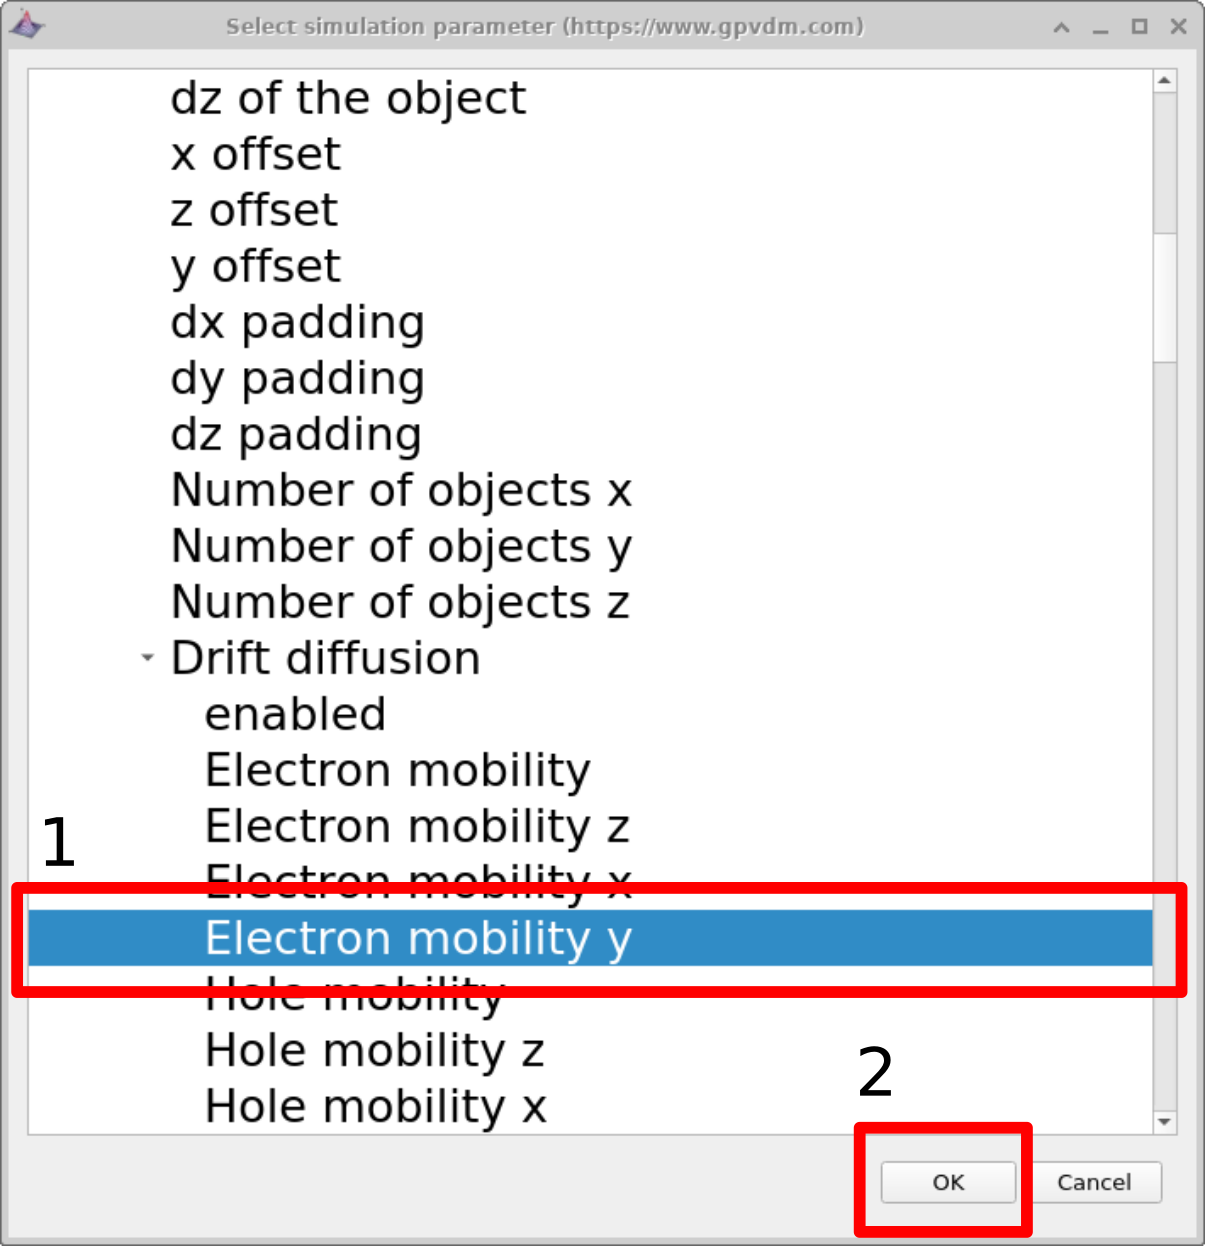
\includegraphics[width=\textwidth]{./images/param_scan_select.png}
\captionof{figure}{Step 5: Select the parameter you want to scan in the parameter selection window, in this case we are selecting epitaxy$\rightarrow$ PM6:Y6$\rightarrow$ Drift diffusion$\rightarrow$ Electron mobility y.}
\label{fig:scanselect}

\end{minipage}

\begin{itemize}

  \item Electron mobility y: One can define asymmetric mobilities in the z,x and y direction - this is useful for OFET simulations.  However by default the model assumes a symmetric mobility which is the same in all directions. This value is defined by \emph{Electron mobility y}. 
\end{itemize}

Next enter the values of mobility which you want to scan over in this case we will be entering \emph{1e-5 1-6 1e-7 1e-8 1e-9} (see figure \ref{fig:runscan} 1) then click \emph{run scan} (see figure \ref{fig:runscan} 2). OghmaNano will run one simulation on each core of your computer until all the simulations are finished.

\begin{figure}[H]
\centering
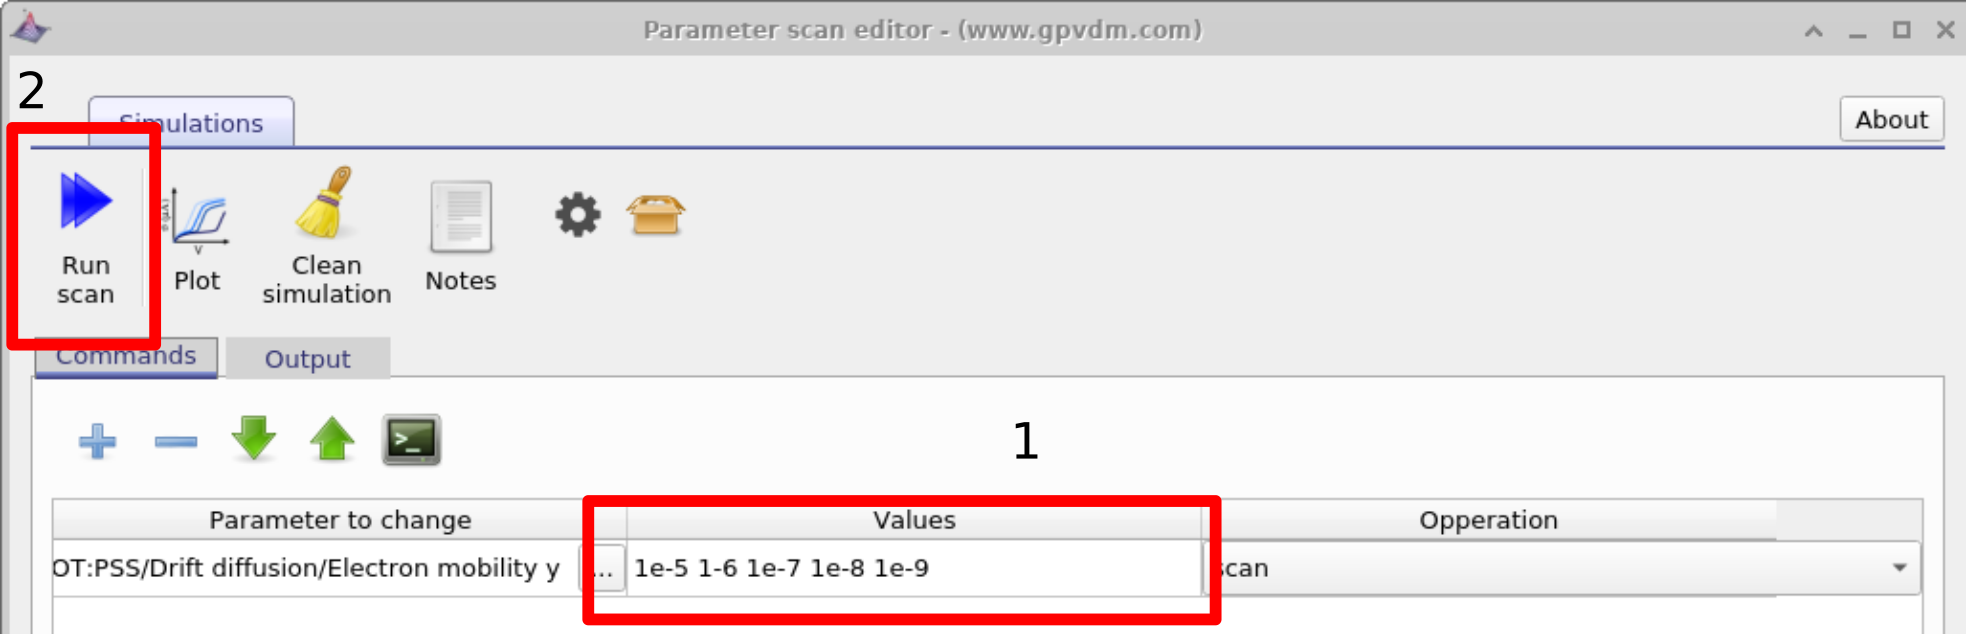
\includegraphics[width=0.8\textwidth]{./images/param_scan_inputvalues.png}
\caption{Step 6: Enter the input values of mobility (or other values) you want to scan over (1). Then run the simulations.}
\label{fig:runscan}
\end{figure}

To view the simulation results click on the \emph{output} tab this will bring up the simulation outputs, see figure \ref{fig:scanoutput}. You can see that a directory has been created for each variable that we scanned over so \emph{1e-5, 1e-6, 1e-7, 1e-8 and 1e-9}.  If you look inside each directory it will be an exact copy of the base simulation directory.  If you double click on the files with multi-colored JV curves, see the red box in figure \ref{fig:scanoutput}. OghmaNano will automaticity plot all the curves from each simulation in one graph, see figure \ref{fig:scanjv}.

\begin{figure}[H]
\centering
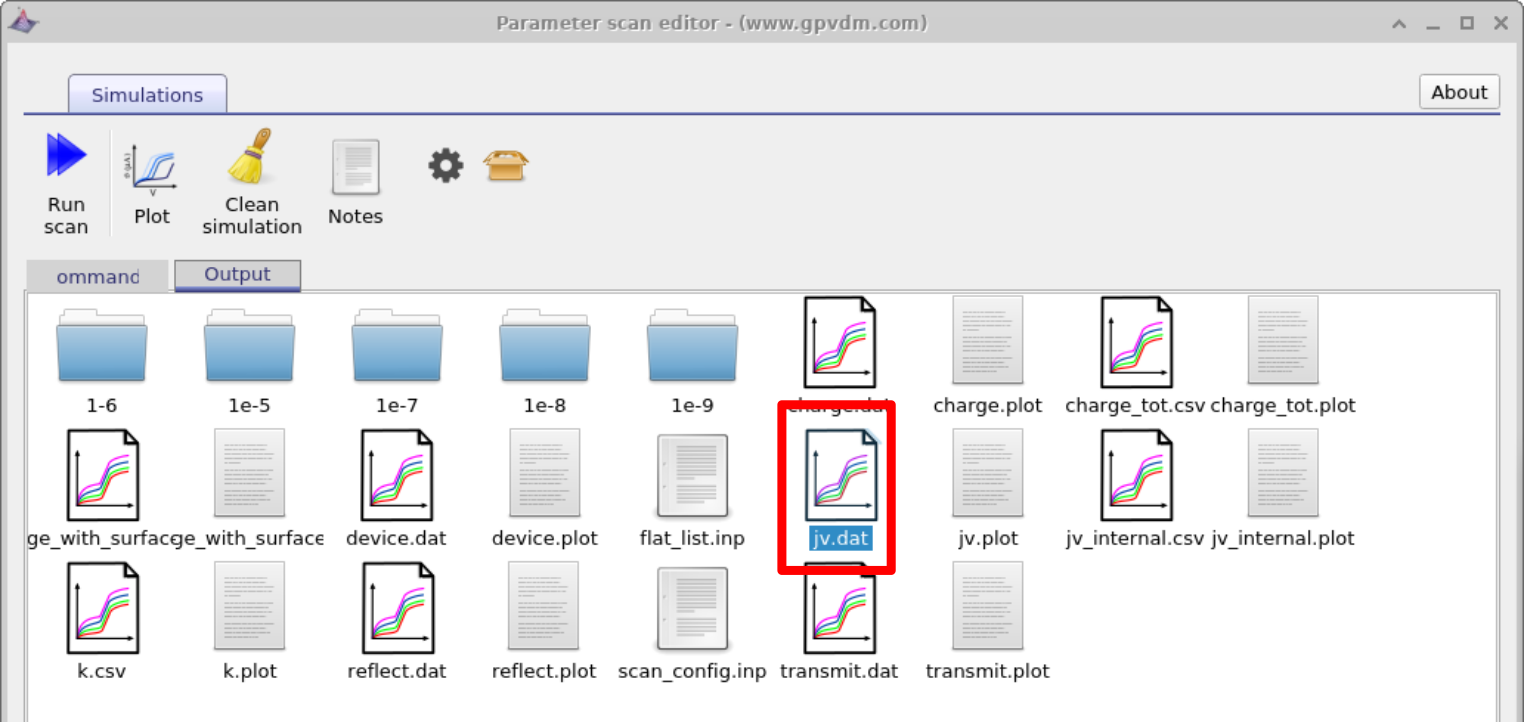
\includegraphics[width=\textwidth]{./images/param_scan_output.png}
\caption{Step 7: The output tab showing the five simulation directories and the multicolored plot files.}
\label{fig:scanoutput}
\end{figure}

\begin{figure}[H]
\centering
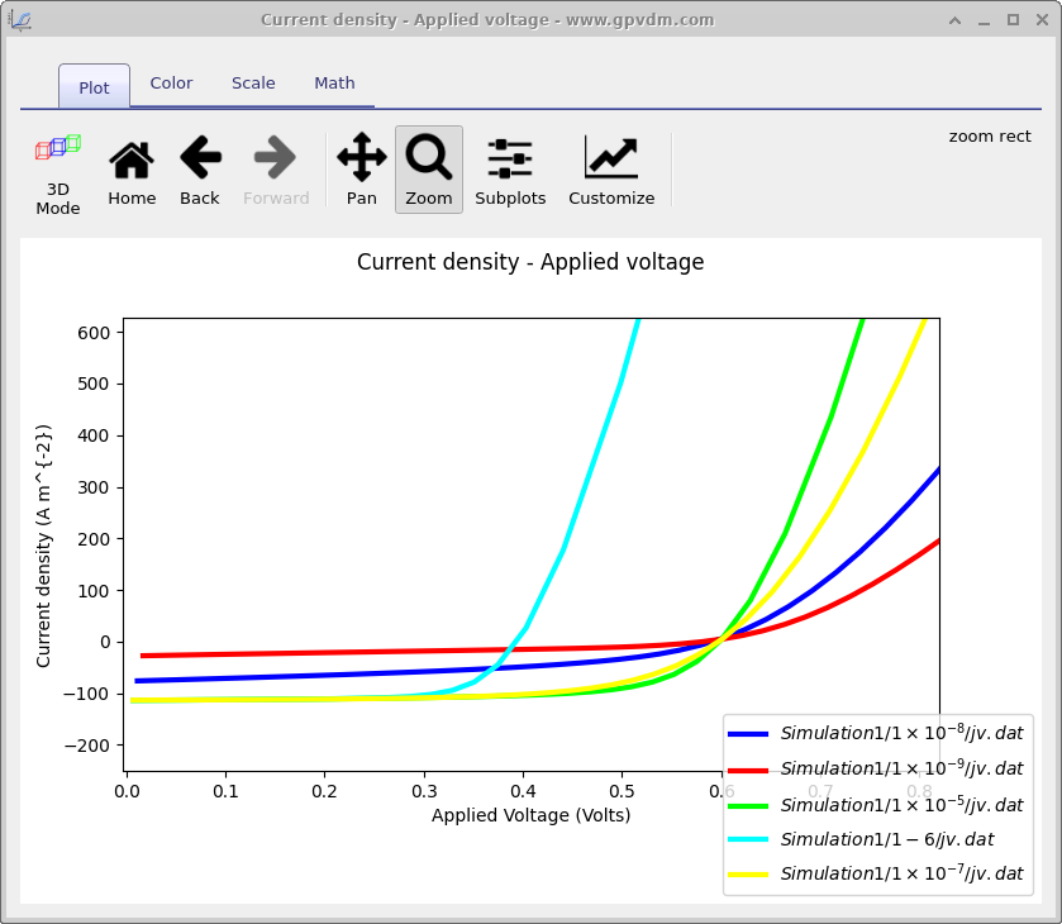
\includegraphics[width=0.5\textwidth]{./images/param_scan_jv.png}
\caption{Step 8: The result of the mobility scan.}
\label{fig:scanjv}
\end{figure}

\subsection{Duplicating parameters - changing the thickness of the active layer}

Very often one wants to change a parameter, then set another parameter equal to the parameter which was changed. An example of this is one may want to change electron and hole mobilities together when simulating a device with symmetric mobilities. This can be done using the duplicate function of the scan window as seen in figure \ref{fig:scanduplicate}.  In this example we tackle a slightly more tricky problem than changing mobilities together we are going to change the physical width of the active layer and at the same time adjust the electrical mesh to make it match.  As discussed in section \ref{ref:mesh} the width of the active layer must always match the width of the electrical mesh.  When you change the layer width by hand in the layer editor OghmaNano updates the width of the electrical mesh for you. But when scripting the model it won't do this update for you.  Therefore in the example below we are going to set the width of the active layer by scanning over:

epitaxy$\rightarrow$PM6:Y6$\rightarrow$dy of the object
\\
\\
Then we are going to add another line under and under parameter to scan select
\\
\\
mesh$\rightarrow$mesh\_y$\rightarrow$segment0$\rightarrow$len
\\
\\
and set it to
\\
\\
epitaxy$\rightarrow$PM6:Y6$\rightarrow$dy of the object
\\
\\
under the operation dropdown box. You will see the word duplicate appear under values.
\\
\\
If you now run the simulation "epitaxy$\rightarrow$PM6:Y6$\rightarrow$dy of the object" will be changed and "mesh$\rightarrow$mesh\_y$\rightarrow$segment0$\rightarrow$len" will follow it.


\begin{figure}[H]
\centering
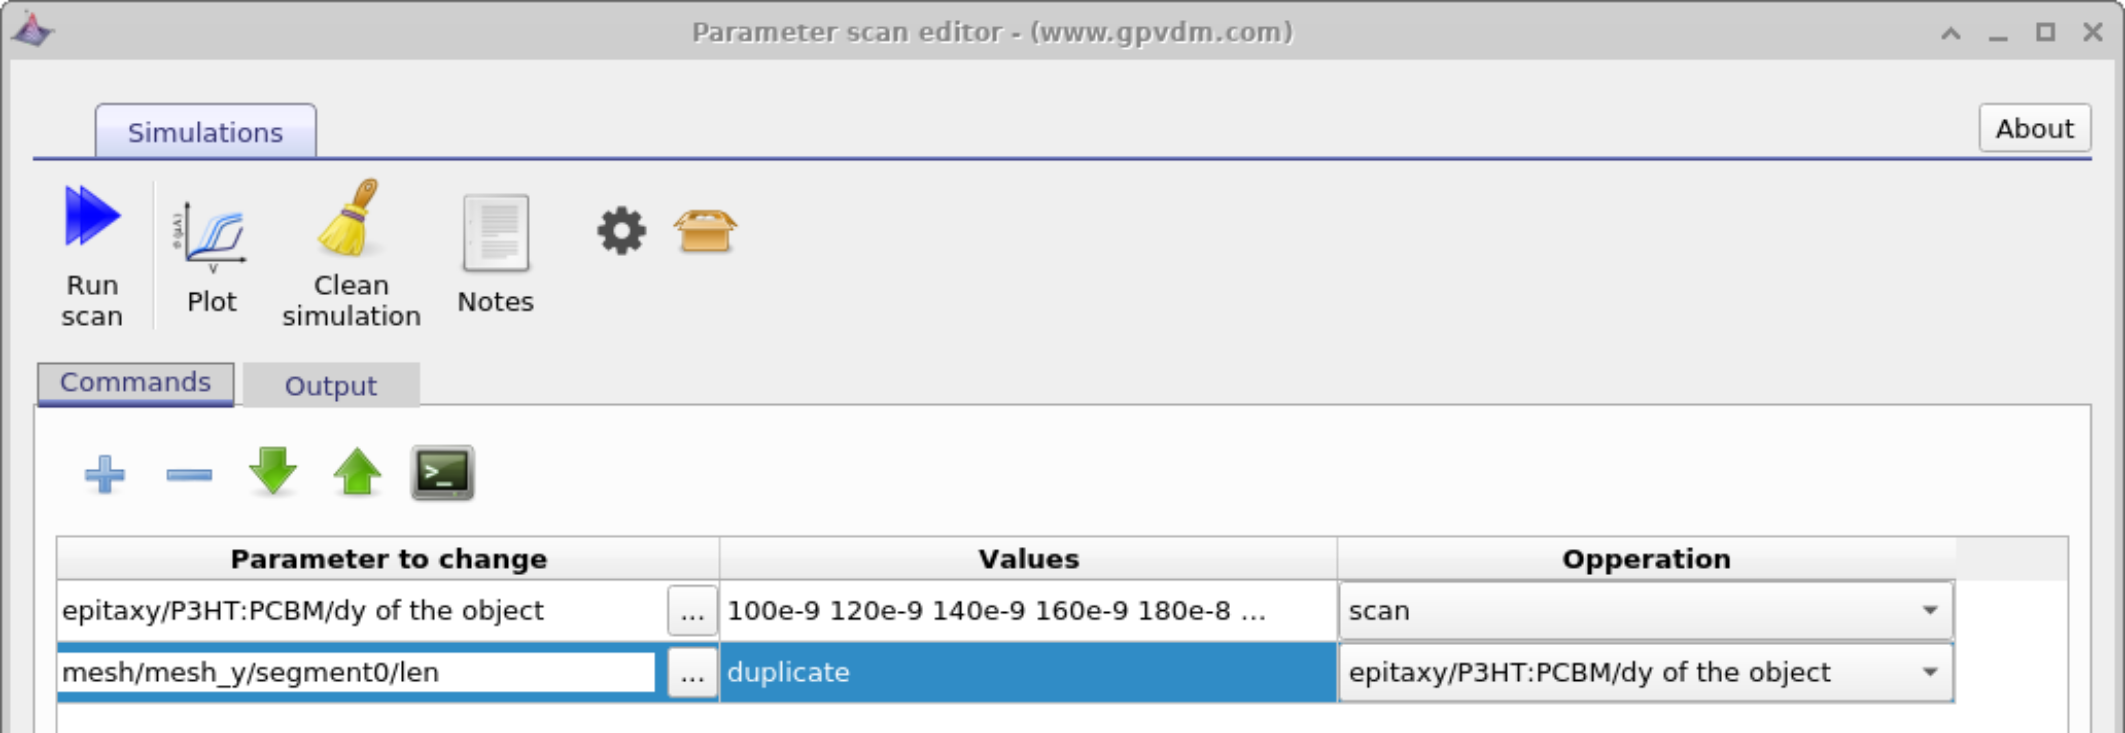
\includegraphics[width=0.7\textwidth]{./images/param_scan_duplicate.png}
\caption{Duplicating material paramters.}
\label{fig:scanduplicate}
\end{figure}

\subsubsection{Side note: Device with multiple active layers}
The sum of the active layer thickness (as defined in the layer editor) MUST equal the electrical mesh thickness (more about the mesh in section \ref{ref:mesh}).  If for example one had three active layers TiO2 (100 nm)/Perovskite (200 nm)/Spiro (100 nm) with a total width of 400 nm.
The total mesh length must be 400 nm as well.  Therefore were one want to change the thickness of the perovskite layer as in \ref{fig:scanduplicate} one would have to break the electrical mesh up into three sections and make sure you were updating the mesh segment referring to the perovskite layer alone.

\subsection{Setting constants}
Often when running a parameter scan one wants to set a constant value, this can be done using the "constant" option in the Operations dropdown menu. See figure \ref{fig:scanconst}

\begin{figure}[H]
\centering
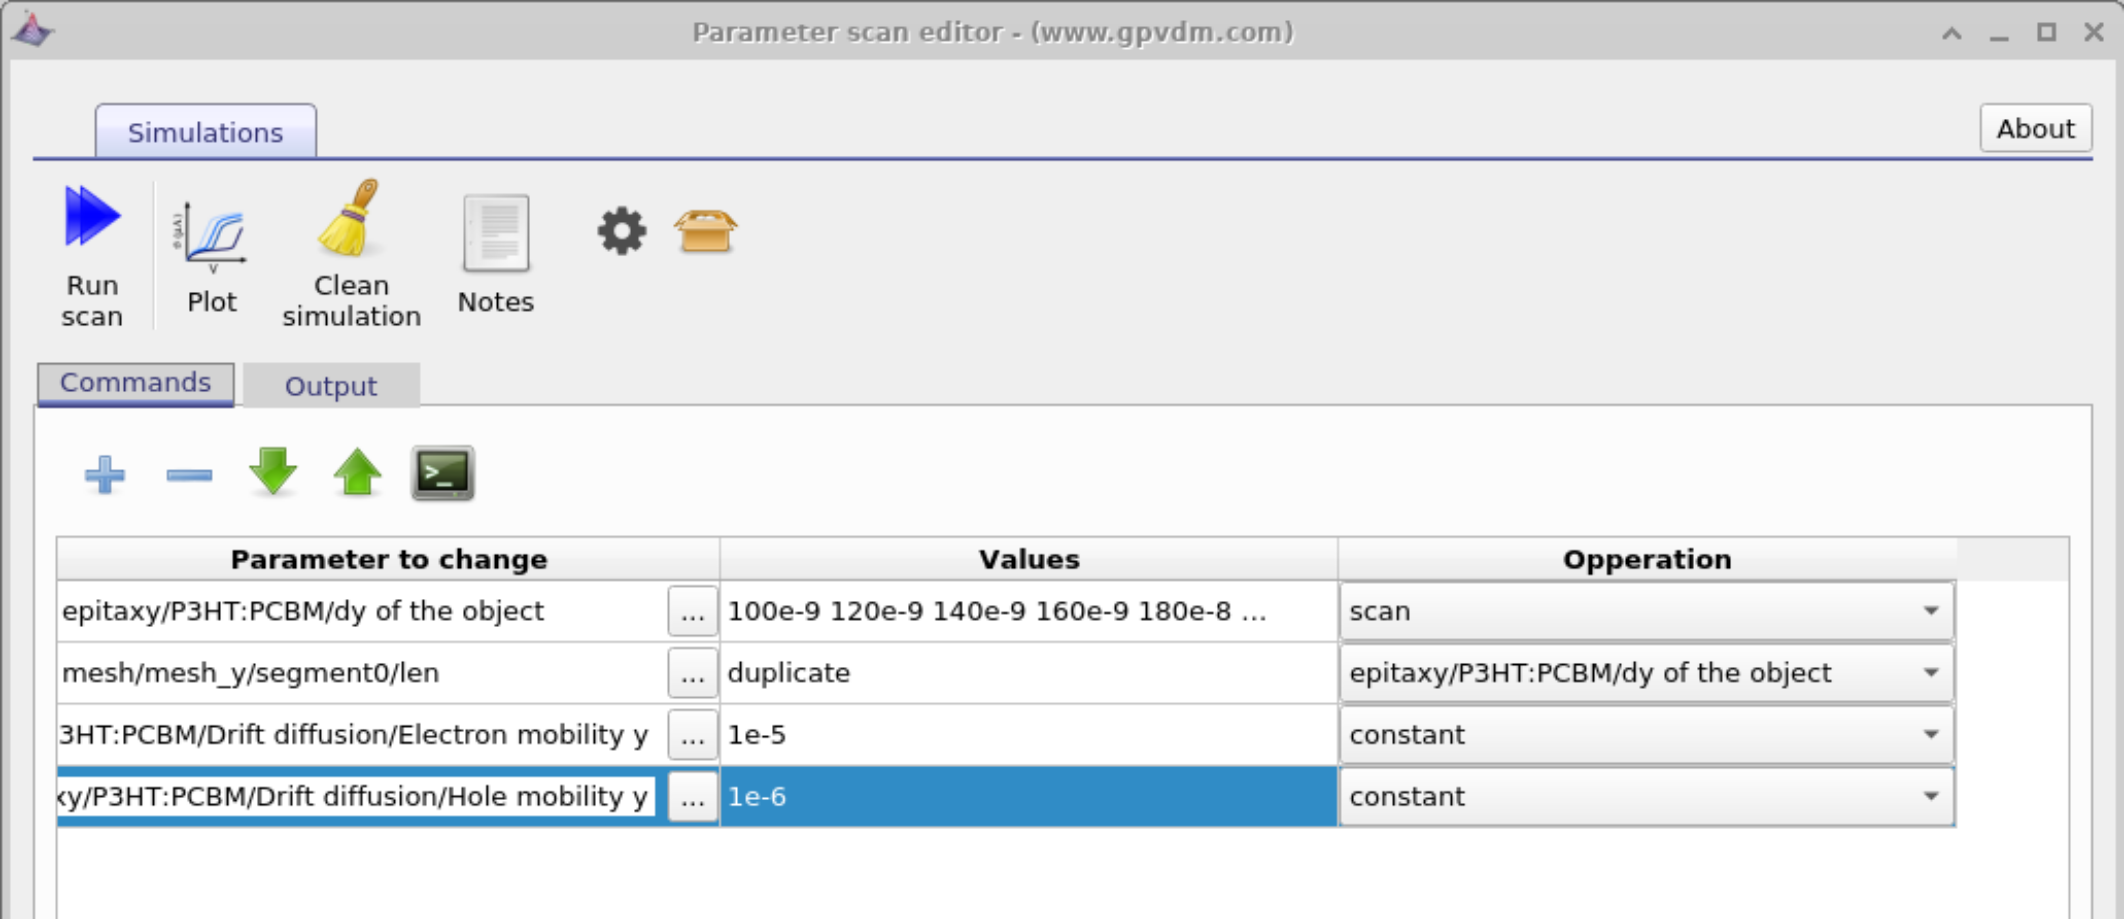
\includegraphics[width=0.5\textwidth]{./images/param_scan_const.png}
\caption{The result of the mobility scan.}
\label{fig:scanconst}
\end{figure}

\subsection{The equivalent of loops}
Often when scanning over a parameter range one may want to simulate so many parameters that it is not practical to type them in.  In this case OghmaNano has the equivalent of a loop. So for example if one wanted to change a value from 100 to 400 in steps of 1, one could type

\begin{listing}[H]
\begin{minted}[frame=single,
               framesep=3mm,
               linenos=false,
               xleftmargin=21pt,
               tabsize=4]{matlab}

[100 400 1]

\end{minted}
\caption{The equivalent of loops in OghmaNano, this is often quicker than typing parameters in by hand.} 
\label{json-example}
\end{listing}

\subsection{Limitations of the scan window}
Although the scan window is convenient in that it provides a quick way to scan simulation parameters, it is by nature rather limited in terms of flexibility. If you want to do complex scans were multiple parameters are changed or to programmatically collect data from each simulation then you can use the \index{python} or matlab interfaces to OghmaNano.  These are described in the latter sections.
\vfill
